\documentclass[12pt]{article}

\usepackage{fancyhdr}
\usepackage{makeidx}
\usepackage[catalan]{babel}
\usepackage{amsfonts}
\usepackage{amssymb}
\usepackage{amsthm}
\usepackage{amsmath}
\usepackage[all]{xy}
\usepackage[ansinew]{inputenc} %%
\usepackage[dvips]{epsfig}
\usepackage{color}



%\usepackage[spanish]{babel}
%\usepackage{color}% usar color para las letras
%\usepackage{graphics}
%\usepackage{graphicx}
%\usepackage{amssymb}
%\usepackage{amsfonts}%para poder poner las letras de Reales Complejos etc...
%\usepackage{anysize} % Soporte para el comando \marginsize
%\usepackage[latin1]{inputenc}% permite poner acentos de forma normal

\setlength{\textwidth}{16cm} \setlength{\textheight}{24cm}
\setlength{\oddsidemargin}{-0.3cm} \setlength{\topmargin}{-1.3cm}

%\usepackage{texfonts}
%\marginsize{2cm}{2cm}{2cm}{2cm}
%\newcommand{\ZZ}{\mathbbmss{Z}}
%\usepackage{fancyhdr}
%\renewcommand{\rmdefault}{phv}
%%%%%%%%%%%%%%%%%%%%%%%%%%%%%%%%%%%%%%%%%%%%%%%%%%%%%%%%%%%%%%%%%%%%%%%%
%-- nuevos comandos para facilitar la escritura
\newcommand{\notacio}{\textbf{Notaci{\'o}}\ \ }
\newcommand{\demostracio}{\textbf{Demostraci{\'o}}\ \ }
\newcommand{\propietats}{\textbf{Propietats}\ \ }
\newcommand{\propietat}{\textbf{Propietat}\ \ }
%\newcommand{\exemple}{\textbf{Exemple}\ \ }
\newcommand{\exemples}{\textbf{Exemples}\ \ }
\newcommand{\observacio}{\textbf{Observaci{\'o}}\ \ }
\newcommand{\observacions}{\textbf{Observacions}\ \ }

\newtheorem{definicio}{Definici{\'o}}[subsection]
\newtheorem{teorema}{Teorema}[subsection]
\newtheorem{Teorema}{Teorema}[subsubsection]
\newtheorem{proposicio}{Proposici{\'o}}[subsection]
\newtheorem{lema}{Lema}[subsection]
\newtheorem{corol}{Corol.lari}[subsection]
\newtheorem{exemple}{Exemple}[subsection]

\newcommand{\Z}{\mathbb{Z}}
\newcommand{\R}{\mathbb{R}}
\newcommand{\C}{\mathbb{C}}
\newcommand{\N}{\mathbb{N}}
\newcommand{\U}{\mathcal{U}}
\newcommand{\V}{\mathcal{V}}
\newcommand{\W}{\mathcal{W}}
\newcommand{\sen}{\mathop{\rm sen}\nolimits}

\begin{document}

\vspace*{7cm}
\begin{center}
\textbf{\Huge{Matem{\`a}tiques II}}

\vspace*{2cm}\textbf{\LARGE{Primer curs}}

\vspace*{2cm}\textbf{\LARGE{Grau en F{\'\i}sica}}

\vspace*{0.6cm}\textbf{\LARGE{Grau en Qu{\'\i}mica}}
\end{center}

\thispagestyle{empty}

\newpage

%\textcolor[rgb]{1.00,1.00,1.00}{palabra} % Pinta "palabra" de blanco
%
%\thispagestyle{empty}
%
%\newpage



\pagenumbering{arabic}

\begin{center}
\section{Introducci{\'o} al c{\`a}lcul d'integrals m{\'u}ltiples}
\end{center}

\parskip =0.3cm
\parindent =0cm
\itemindent=2cm

En aquest tema estudiarem el concepte d'integraci{\'o} de funcions reals
amb v{\`a}ries variables. M{\'e}s concretament ens limitarem
%b{\`a}sicament
a funcions de dues variables.
% i a alguns exemples de funcions amb tres
%variables.
Veurem que la integraci{\'o} m{\'u}ltiple {\'e}s una generalitzaci{\'o} a
v{\`a}ries variables del concepte d'integraci{\'o} per una variable
introdu{\"\i}t en la assignatura de Matem{\`a}tiques I.

\vspace*{1cm}
\subsection{Integral doble en dominis rectangulars}

Per introduir la definici{\'o} d'integral doble necessitam uns conceptes
preliminars.

\begin{definicio}
Sigui $\, R=[a,b]\times[c,d]\,$ un rectangle de $\R^2$. Direm
\textbf{partici{\'o} regular d'ordre n} del rectangle $R$ a dues
col.leccions de $n+1$ punts equidistants $\,\{x_i\}, \, \{y_i\}, \ \
i=0,\ldots
,n\,$ que verifiquen:\\

\hspace{3cm}$a=x_0<x_1<\cdots x_n=b\,,\quad
x_{i+1}-x_i=\frac{b-a}{n}=\triangle x\ $ (increment de $x$).\\

\hspace{3cm}$c=y_0<y_1<\cdots y_n=d\,,\quad
y_{i+1}-y_i=\frac{d-c}{n}=\triangle y\ $ (increment de $y$).\\

Queden determinats $n^2$ rectangles petits: $\
R_{ij}=[x_i,x_{i+1}]\times[y_j,y_{j+1}]\,,\ i,j=0,\ldots,n-1\,$.
\end{definicio}

%*********************************************************************
\vspace*{4cm}
\begin{center}
\begin{picture}(0,0)(130,30)
\resizebox{8cm}{!}{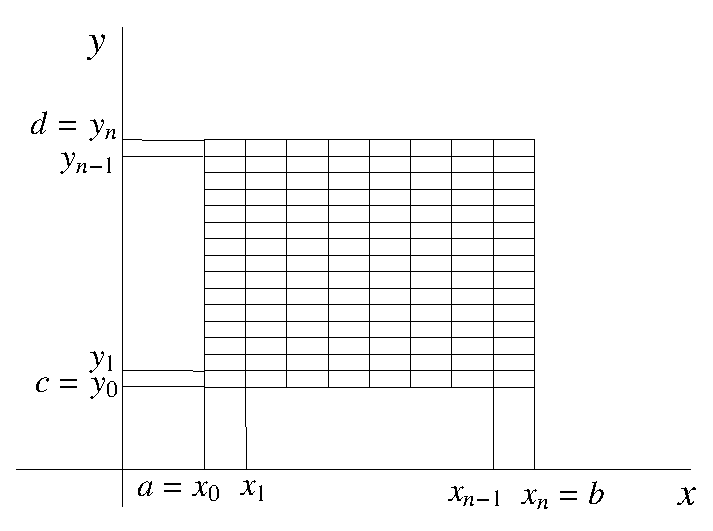
\includegraphics{fig1.eps}}
\end{picture}
\end{center}

%*********************************************************************
\vspace*{2cm}

\begin{definicio}
Siguin $\, f:A\to \R\,,$  $R$ un rectangle tal que $R\subset
A\subset\R^2$ i $R_{ij}$ una partici{\'o} regular de $R$ d'ordre n.
Definim \textbf{suma de Riemann de f associada a la partici{\'o}} com:\\

\hspace{3cm}$s_n=\displaystyle \sum\limits_{i,j=0}^{n-1}\, f(c_{ij})
\triangle x\triangle y\,,\qquad c_{ij}\in R_{ij}$. \\
\end{definicio}

%%*********************************************************************
\vspace*{4cm}
\begin{center}
\begin{picture}(0,0)(130,30)
\resizebox{10cm}{!}{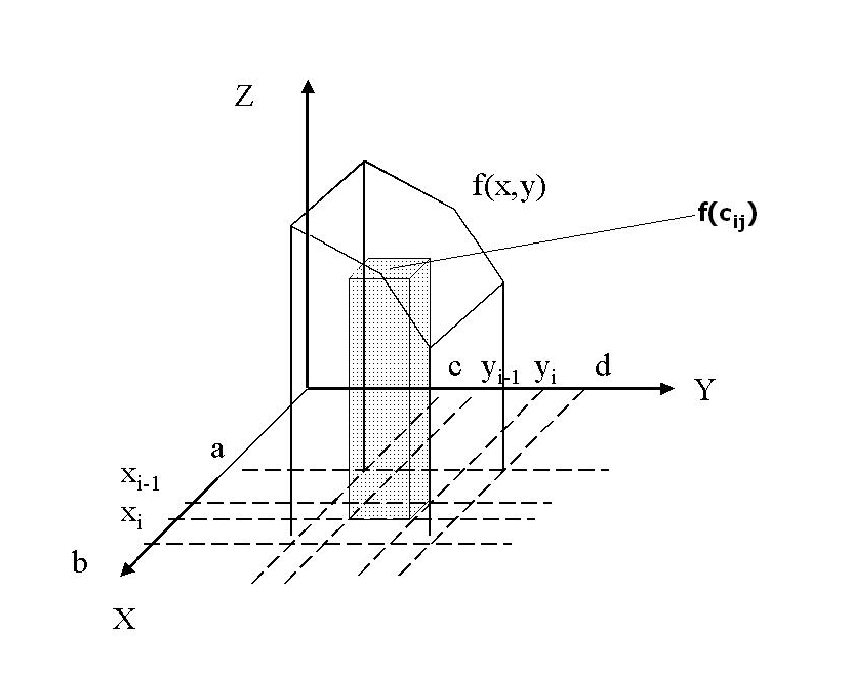
\includegraphics{fig2.eps}}
\end{picture}
\end{center}

%%*********************************************************************
\vspace*{1cm}

\begin{observacio}
De la definici{\'o} anterior s'observa clarament que la suma de Riemann
dep{\`e}n de l'el.lecci{\'o} de $c_{ij}$ dins el rectangle $R_{ij}$.
\end{observacio}


Ara ja podem donar la definici{\'o} d'integral.

\begin{definicio}
Si la successi{\'o} $\{s_n\}$ de sumes de Riemann t{\'e} l{\'\i}mit i {\'e}s
independent de l'ele.lecci{\'o} dels $c_{ij}\in R_{ij}$, direm que
\textbf{f {\'e}s integrable en R} i el valor de la integral {\'e}s aquest
l{\'\i}mit.
\end{definicio}

\textbf{Notaci{\'o}} Es poden util.litzar les seg{\"u}ents notacions per a
representar una integral doble:\\

\hspace{1cm}$\displaystyle \int\!\!\!\int_R\,f(x,y)\,dx\,dy\,;\qquad
\int_R\,f(x,y)\,dx\,dy\,;\qquad\int_R\,f(x,y)\,dA\,; \qquad \int_R\,f\,dx\,dy$\\

\begin{observacio}
Si la funci{\'o} $f$ verifica que $\,f(x,y)\geq 0\, \ \forall(x,y)\in
R$, la seva integral {\'e}s el volum del s{\`o}lid de base $R$ limitat
superiorment per la gr{\`a}fica de $f$ i lateralment pels plans $x=a,\,
x=b,\, y=c,\, y=d$.
\end{observacio}

%%*********************************************************************
\vspace*{7cm}
\begin{center}
\begin{picture}(0,0)(130,30)
\resizebox{10cm}{!}{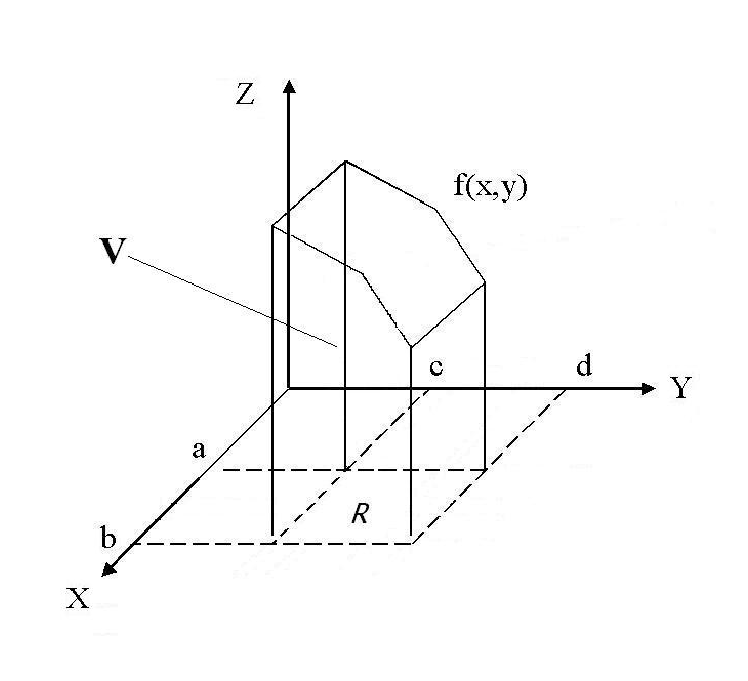
\includegraphics{fig3.eps}}
\end{picture}
\end{center}

%%*********************************************************************
\vspace*{-1cm}

 A partir d'aquestes definicions i de
certes propietats de les funcions de varies variables, es poden
obtenir els seg{\"u}ents resultats.

\begin{teorema}
Tota funci{\'o} cont{\'\i}nua en el rectangle $R$ {\'e}s integrable.
\end{teorema}

\begin{teorema}
Siguin $f$ i $g$ dues funcions integrables en $R$ i sigui $c\in\R$
una constant, llavors:\\

a) $f+g\,$ {\'e}s integrable en $R$. Es verifica $\ \displaystyle
\int_R\,(f+g)\,dx\,dy= \int_R\,f\,dx\,dy\,+ \int_R\,g\,dx\,dy$\\

b) $c\,f\,$ {\'e}s integrable en $R$. Es verifica $\ \displaystyle
\int_R\,(c\,f)\,dx\,dy= c\int_R\,f\,dx\,dy$
\end{teorema}

\begin{teorema}
Sigui $R$ un rectangle tal que $\,R=R_1\cup R_2\cup\cdots\cup R_m\,$
on $R_i$ s{\'o}n rectangles que  tenen en com{\'u} com a molt un costat. Es
verifica que si $f$ {\'e}s integrable per a cada $R_i\,,\ \
i=1,\ldots,m\,,$ llavors $f$ {\'e}s integrable en $R$. Es compleix que\\

\hspace{3cm}$\displaystyle
\int_R\,f\,dA=\sum\limits_{i=1}^m\int_{R_i}\,f\,dA$
\end{teorema}

\begin{teorema}
Siguin $f$ i $g$ dues funcions integrables en $R$ tals que
$\,f(x,y)\leq g(x,y)$

$\forall (x,y)\in R\,.$ Llavors\\

\hspace{3cm}$\displaystyle \int_R\,f\,dA\leq\int_R\,g\,dA$
\end{teorema}

El seg{\"u}ent resultat conegut com el \textbf{Teorema de Fubini} {\'e}s
molt interessant ja que ens permetr{\`a} calcular les integrals dobles
com a integrals d'una variable que ja sabem fer.

\begin{teorema}
Sigui $R$ el rectangle $\, R=[a,b]\times[c,d]\,$ i $\, f:R\to \R\,,$
una funci{\'o} cont{\'\i}nua. Aleshores\\

\hspace{3cm}$\displaystyle
\int_R\,f\,dA=\int_a^b\left(\int_c^d\,f(x,y)\,dy\right)dx=
\int_c^d\left(\int_a^b\,f(x,y)\,dx\right)dy$
\end{teorema}

\begin{observacio}
Existeixen funcions integrables que no s{\'o}n cont{\'\i}nues a les quals
tamb{\'e} {\'e}s pot aplicar el teorema de Fubini.
\end{observacio}

\begin{exemple}
Sigui $R=[0,1]\times[0,1]$. Calculau $I=\displaystyle\int_R(x^3 y
-\sqrt{x y})dx\, dy\,.$
\end{exemple}

Com que la funci{\'o} $\,f(x,y)=x^3 y -\sqrt{x y}\,$ {\'e}s cont{\'\i}nua en $R$
podem aplicar el teorema de Fubini per calcular la integral. Ho
podem fer de dues maneres (evidentment basta fer-ne una de les
dues):\\

\hspace*{1cm}\textbf{1.}$\displaystyle\ \
I=\int_0^1\left(\int_0^1(x^3 y -\sqrt{x y})dx\right)dy=
\int_0^1\left[\frac{x^4 y}{4} -\frac{2}{3}x\sqrt{x
y}\right]_0^1\,dy=$\\

\hspace*{1cm}$\displaystyle\ \ \ \ \int_0^1(\frac{y}{4}
-\frac{2}{3}\sqrt{ y})\,dy=\left[\frac{y^2}{8}
-\left(\frac{2}{3}\right)^2 y\sqrt{
y}\right]_0^1=-\frac{23}{72}\,.$\\ \\

\hspace*{1cm}\textbf{2.}$\displaystyle\ \
I=\int_0^1\left(\int_0^1(x^3 y -\sqrt{x y})dy\right)dx=
\int_0^1\left[\frac{x^3 y^2}{2} -\frac{2}{3}y\sqrt{x
y}\right]_0^1\,dx=$\\

\hspace*{1cm}$\displaystyle\ \ \ \ \int_0^1(\frac{x^3}{2}
-\frac{2}{3}\sqrt{x})\,dx=\left[\frac{x^4}{8}
-\left(\frac{2}{3}\right)^2 x\sqrt{
x}\right]_0^1=-\frac{23}{72}\,.$\\\\

\begin{exemple}
Calculau el volum del s{\`o}lid limitat per la superf{\'\i}cie $\,z=x^2+y^2\,
$ i el rectangle $\, R=[-1,1]\times[-1,1]\, $.
\end{exemple}

%*********************************************************************
\vspace*{5cm}
\begin{center}
\begin{picture}(0,0)(130,30)
\resizebox{10cm}{!}{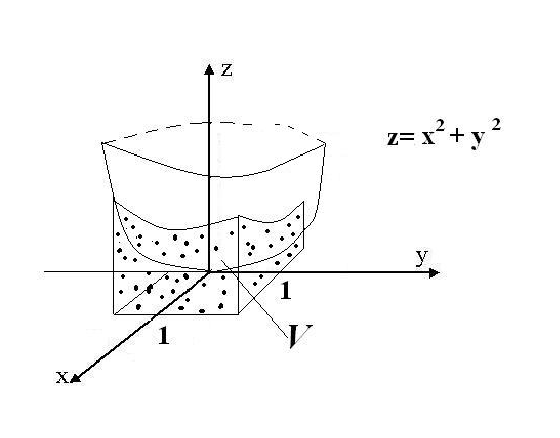
\includegraphics{fig4-a.eps}}
\end{picture}
\end{center}

%*********************************************************************
\vspace*{1cm}

Com que la funci{\'o} $\, f(x,y)=x^2+y^2\, $ {\'e}s tal que $\, f\geq 0\, $
en $R$, llavors el volum se pot obtenir fent $\, \displaystyle\int_R
\, f\, dA\, $ i ja que $f$ {\'e}s cont{\'\i}nua, podem aplicar el teorema de
Fubini:\\

\hspace*{1cm}$\displaystyle\ \
V=\int_{-1}^1\left(\int_{-1}^1(x^2+y^2)dx\right)dy=
\int_{-1}^1\left[\frac{x^3}{3} +x
y^2\right]_{-1}^1\,dy=\int_{-1}^1(\frac{2}{3}
+2y^2)\,dy=$\\

\hspace*{1cm}$\displaystyle\ \ \ \ \left[\frac{2}{3}y
+\frac{2}{3}y^3\right]_{-1}^1=\frac{8}{3}\,.$

\vspace*{1cm}
\subsection{Integraci{\'o} en dominis m{\'e}s generals}

Donarem ara una definici{\'o} que ens permetr{\`a} considerar la integral
doble sobre regions m{\'e}s generals que els rectangles abans
considerats.

\begin{definicio}
Sigui $D$ un subconjunt de $\R^2$ que est{\`a} fitat. Sigui
$\,f:D\to\R\,$ una funci{\'o} que {\'e}s integrable sobre un rectangle $R$
tal que $\,D\subset R\,.$ Podem estendre $f$ en tot el rectangle $R$
de la manera seg{\"u}ent:\\

\hspace*{3cm}$f_1(x,y)=\left\{\begin{array}{ll}
              f(x,y) & \mbox{si $\ \ (x,y)\in D$}\\
               & \\
               0  & \mbox{si $\ \ (x,y)\not\in D$}
             \end{array} \right .$\\\\

Llavors definim $\
\displaystyle\int_D\,f(x,y)\,dA=\int_R\,f_1(x,y)\,dA\,.$
\end{definicio}

%*********************************************************************
\vspace*{6cm}
\begin{center}
\begin{picture}(0,0)(130,30)
\resizebox{9.5cm}{!}{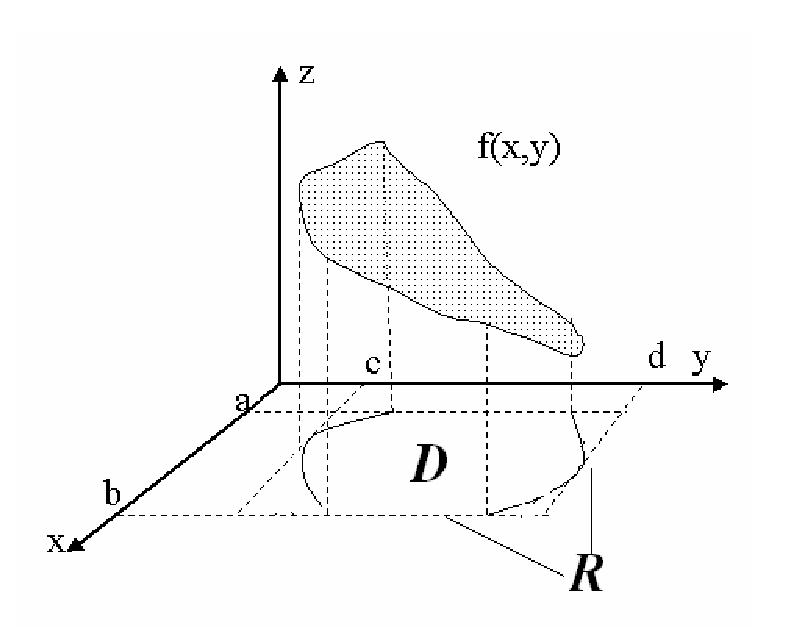
\includegraphics{fig4.eps}}
\end{picture}
\end{center}

%*********************************************************************
\vspace*{1cm}

Consideram tres tipus de dominis en $\R^2$. (Un domini {\'e}s un conjunt
fitat i obert).

\textbf{Domini de tipus 1.} Siguin $\,\phi_1,\,\phi_2:[a,b]\to\R\,$
dues funcions cont{\'\i}nues. $D$ {\'e}s un domini de tipus 1 si {\'e}s de la
forma:
$$ D=\{(x,y)\in\R^2\ :\ a\leq x\leq b,\ \ \phi_1(x)\leq y\leq \phi_2(x)\}$$

%*********************************************************************
\vspace*{3cm}
\begin{center}
\begin{picture}(0,0)(70,30)
\resizebox{6cm}{!}{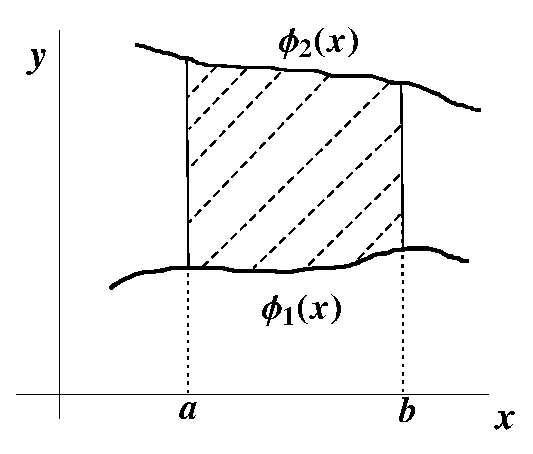
\includegraphics{fig5-1.eps}}
\end{picture}
\end{center}

%*********************************************************************
\vspace*{1cm}

\textbf{Domini de tipus 2.} Siguin $\,\psi_1,\,\psi_2:[c,d]\to\R\,$
dues funcions cont{\'\i}nues. $D$ {\'e}s un domini de tipus 2 si {\'e}s de la
forma:
$$ D=\{(x,y)\in\R^2\ :\ c\leq y\leq d,\ \ \psi_1(y)\leq x\leq \psi_2(y)\}$$

%*********************************************************************
\vspace*{3cm}
\begin{center}
\begin{picture}(0,0)(70,30)
\resizebox{6cm}{!}{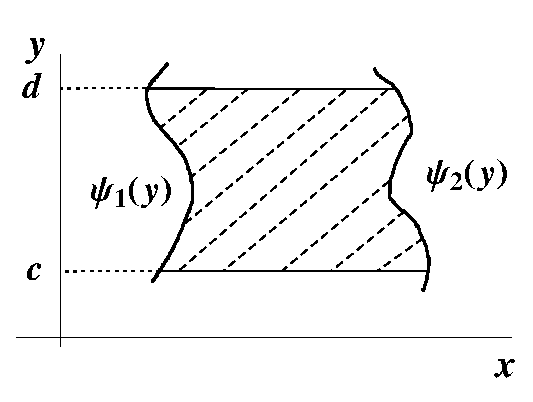
\includegraphics{fig5-2.eps}}
\end{picture}
\end{center}

%*********************************************************************
\vspace*{1cm}

\textbf{Domini de tipus 3.} Direm que $D$ {\'e}s un domini de tipus 3 si
{\'e}s de tipus 1 i de tipus 2 a la vegada.

\begin{observacio}
Conv{\'e} notar que hi ha regions que no s{\'o}n de cap dels tipus anteriors
per{\`o} que es poden descompondre en trossos que s{\'\i} ho s{\'o}n, per exemple
la regi{\'o} $D$ donada per:


%*********************************************************************
\vspace*{3cm}
\begin{center}
\begin{picture}(0,0)(70,30)
\resizebox{5cm}{!}{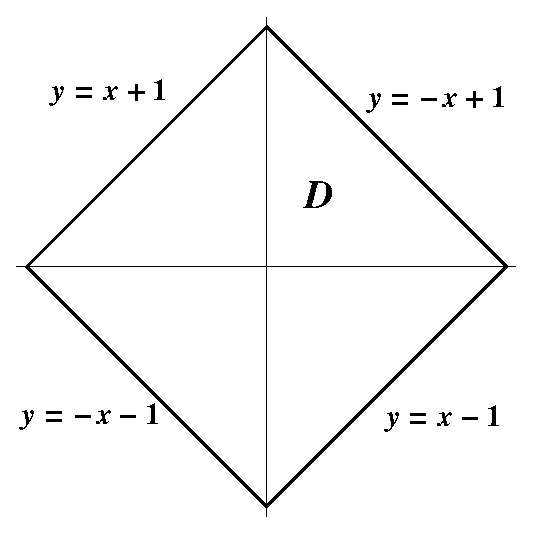
\includegraphics{fig12.eps}}
\end{picture}
\end{center}

%*********************************************************************
\vspace*{1cm}

es pot descompondre amb dues regions de tipus 1:

%*********************************************************************
\vspace*{4.5cm}
\begin{center}
\begin{picture}(0,0)(170,30)
\resizebox{5cm}{!}{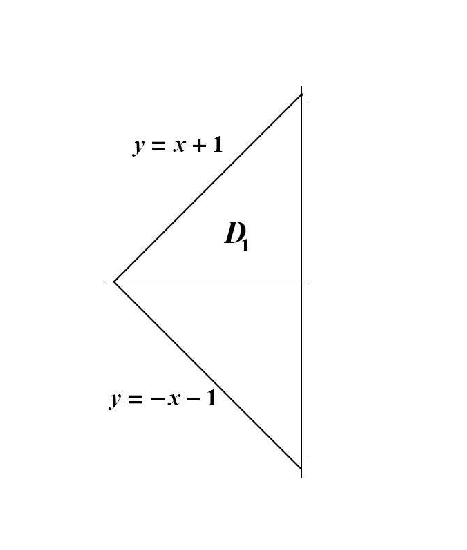
\includegraphics{figura12-1.eps}}\hspace{2cm}
\resizebox{4.5cm}{!}{\includegraphics{figura12-2.eps}}
\end{picture}
\end{center}

%*********************************************************************
%\vspace*{2cm}

 o dues regions de tipus 2:

%*********************************************************************
\vspace*{1.5cm}
\begin{center}
\begin{picture}(0,0)(170,30)
\resizebox{5cm}{!}{\includegraphics{figura12-3.eps}}\hspace{2cm}
\resizebox{5.4cm}{!}{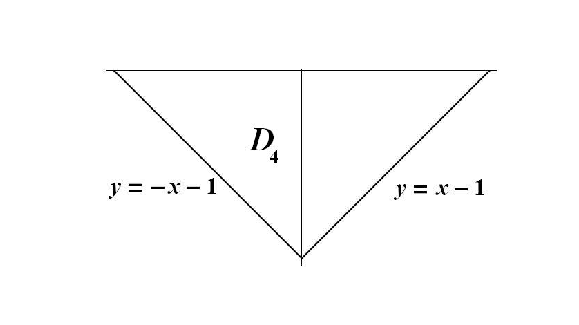
\includegraphics{figura12-4.eps}}
\end{picture}
\end{center}

%*********************************************************************
\vspace*{1.5cm}

\end{observacio}

El seg{\"u}ent resultat  basat en el teorema de Fubini ens proporciona
un m{\`e}tode per a calcular integrals sobre aquests dominis.

\begin{teorema}
a) Sigui $D$ un domini de tipus 1 i $\,f:D\to \R\,$ una funci{\'o}
cont{\'\i}nua. Aleshores\\

\hspace*{3cm}$\displaystyle\int_D\,f(x,y)\,dA=
\int_a^b\left(\int_{\phi_1(x)}^{\phi_2(x)}\,f(x,y)\, dy\right)dx$\\

b) Sigui $D$ un domini de tipus 2 i $\,f:D\to \R\,$ una funci{\'o}
cont{\'\i}nua. Aleshores\\

\hspace*{3cm}$\displaystyle\int_D\,f(x,y)\,dA=
\int_c^d\left(\int_{\psi_1(y)}^{\psi_2(y)}\,f(x,y)\, dx\right)dy$\\
\end{teorema}

Un resultat que {\'e}s conseq{\"u}{\`e}ncia immediata d'aquest teorema {\'e}s el
seg{\"u}ent corol.lari.

\begin{corol}
L'{\`a}rea d'un domini $D$ es pot calcular per la seg{\"u}ent integral:\\

\hspace*{3cm}$\displaystyle\int_D\,1\,dA\,.$
\end{corol}

\begin{exemple}
Calculau $\ \displaystyle\int_T\,(x^3y+\cos x)\,dA\ $ on $T$ {\'e}s el
triangle de v{\`e}rtexs $(0,0), (\pi/2,0)\ $ i $(\pi/2,\pi/2).$
\end{exemple}

%*********************************************************************
\vspace*{2.5cm}
\begin{center}
\begin{picture}(0,0)(130,30)
\resizebox{4.5cm}{!}{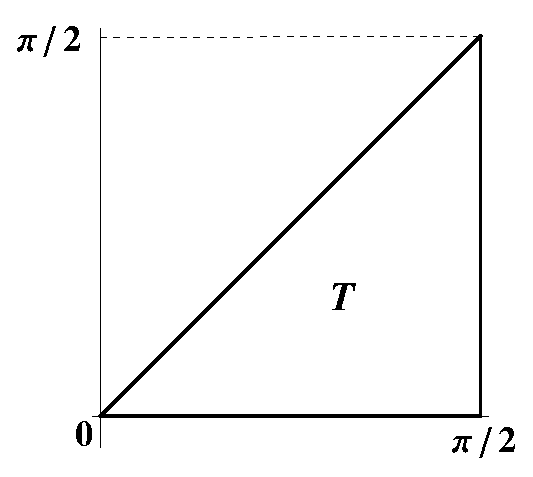
\includegraphics{fig6.eps}}
\end{picture}
\end{center}

%*********************************************************************
\vspace*{1cm}

El triangle $T$ ho podem escriure com $\ T=\{(x,y)\in\R^2\ :\ 0\leq
x\leq \pi/2,\ \ 0\leq y\leq x\}\,.$ Per tant {\'e}s un domini de tipus
1. Aleshores\\

\hspace*{1cm}$\displaystyle\int_T\,(x^3y+\cos x)\,dA=
\int_0^{\pi/2}\left(\int_{0}^{x}\,(x^3y+\cos x)\,
dy\right)dx=\int_0^{\pi/2}\left[\frac{x^3 y^2}{2}+ y\cos
x\right]_0^xdx=$\\\\

\hspace*{1cm}$\displaystyle\int_0^{\pi/2}\left(\frac{x^5}{2}+ x\cos
x\right)dx=\left[\frac{x^6}{12}+ x\sin x+\cos
x\right]_0^{\pi/2}=\frac{\pi^6}{768}+\frac{\pi}{2}-1$\\


\begin{exemple}
Calculau el volum del tetraedre limitat pels plans $\ x=0,y=0,z=0\ $
i $\ z=1+x-y\,.$
\end{exemple}

Si feim $\,z=0\,$ a l'equaci{\'o} del pla $\, z=1+x-y\,$ obtenim la
recta $\ 1+x-y=0\,.$ Llavors el domini $D$ ho podem escriure com $\
D=\{(x,y)\in\R^2\ :\ 0\leq y\leq 1,\ \ y-1\leq x\leq 0\}\,.$

%*********************************************************************
\vspace*{3.5cm}
\begin{center}
\begin{picture}(0,0)(70,30)
\resizebox{4.5cm}{!}{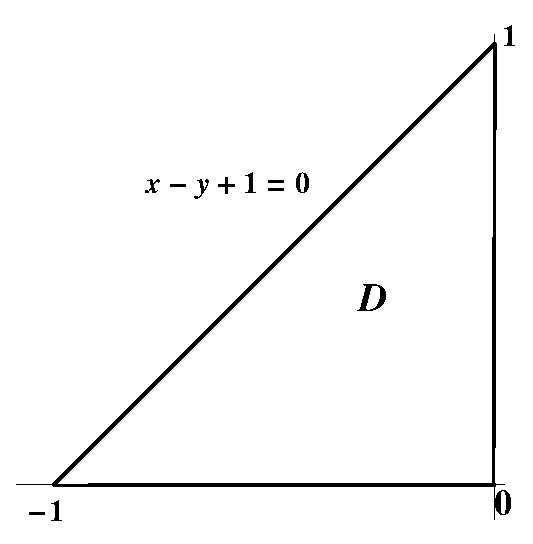
\includegraphics{fig7.eps}}
\end{picture}
\end{center}

%*********************************************************************
\vspace*{1cm}

Per tant {\'e}s un domini de tipus 2. Aleshores\\

\hspace*{1cm}$\displaystyle\int_D\,(1+x-y)\,dA=
\int_0^{1}\left(\int_{y-1}^{0}\,(1+x-y)\,
dx\right)dy=\int_0^{1}\left[x+\frac{x^2}{2}-yx\right]_{y-1}^0dy=$\\\\


\hspace*{1cm}$\displaystyle\frac{1}{2}\int_0^{1}(y^2-2y
+1)dy=\frac{1}{2}\left[\frac{y^3}{3}-y^2+y\right]_0^{1}=\frac{1}{6}$\\

\begin{observacio}
Com {\'e}s evident, els dominis de tipus 3 es poden integrar utilitzant
qualsevol de les dues possibilitats donades al teorema anterior.
\end{observacio}

\begin{exemple}
Calculau $\ \displaystyle\int_D\,y(1-\cos x)\,dA\ $ on $D$ {\'e}s el
domini limitat per $\ x=0,y=2\ $ i $\ y=\sqrt{x}\,.$
\end{exemple}

%*********************************************************************
\vspace*{1.2cm}
\begin{center}
\begin{picture}(0,0)(150,30)
\resizebox{6cm}{!}{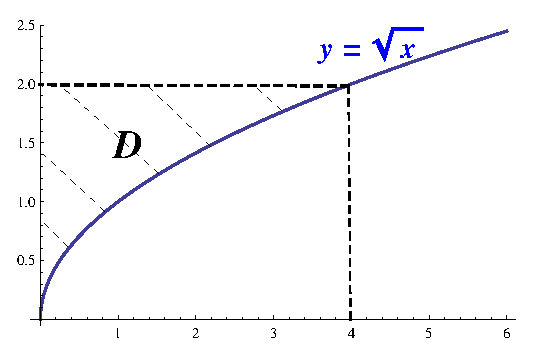
\includegraphics{fig8.eps}}
\end{picture}
\end{center}

%*********************************************************************
\vspace*{1cm}

El domini $D$ {\'e}s un domini de tipus 3 ja que ho podem escriure com:\\

$\ D=\{(x,y)\in\R^2\ :\ 0\leq x\leq 4,\ \ \sqrt{x}\leq y\leq 2\}\,$
(domini de tipus 1).\\

$\ D=\{(x,y)\in\R^2\ :\ 0\leq y\leq 2,\ \ 0\leq x\leq y^2\}\,$
(domini de tipus 2).\\

Podem calcular la nostra integral de dues maneres:\\

\hspace*{1cm}$\displaystyle\int_D\,y(1-\cos x)\,dA=
\int_0^{4}\left(\int_{\sqrt{x}}^{2}\,y(1-\cos x)\,
dy\right)dx=\int_0^{4}\left[\frac{y^2}{2} (1- \cos x)\right]_{\sqrt{x}}^{2}dx=$\\\\


\hspace*{1cm}$\displaystyle\int_0^{4}\left(2-\frac{x}{2}\right)\left(1-\cos
x\right)dx=\left[2x-\frac{x^2}{4}-2\sin
x+\frac{1}{2}(\cos x+x\sin x)\right]_0^{4}=\frac{7}{2}+\frac{\cos 4}{2}$\\

O tamb{\'e}\\

\hspace*{1cm}$\displaystyle\int_D\,y(1-\cos x)\,dA=
\int_0^{2}\left(\int_{0}^{y^2}\,y(1-\cos x)\,
dx\right)dy=\int_0^{2}[yx -y\sin x]_0^{y^2}dy=$\\\\


\hspace*{1cm}$\displaystyle\int_0^{2}(y^3-y \sin
y^2)dy=\left[\frac{y^4}{4}+\frac{1}{2}\cos
y^2\right]_0^{2}=\frac{7}{2}+\frac{\cos 4}{2}$\\\\

De fet si estam integrant en dominis de tipus 3 a vegades potser
molt interessant fer un canvi d'ordre d'integraci{\'o} per facilitar els
c{\`a}lculs.\\

\begin{exemple}
Calculau $\ \displaystyle
I=\int_0^a\left(\int_0^{\sqrt{a^2-x^2}}\sqrt{a^2-y^2}\,dy\right)dx\qquad
a>0\,.$
\end{exemple}

%*********************************************************************
\vspace*{3cm}
\begin{center}
\begin{picture}(0,0)(70,30)
\resizebox{4cm}{!}{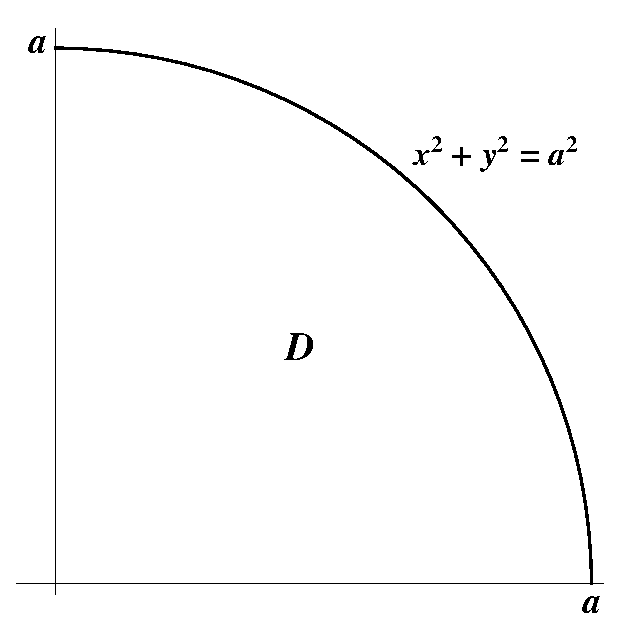
\includegraphics{fig9.eps}}
\end{picture}
\end{center}

%*********************************************************************
\vspace*{1cm}

Per calcular $I$ tendr{\'\i}em primer que trobar una primitiva de la
funci{\'o} $\ f(y)=\sqrt{a^2-y^2}\ $. Per fer-ho consideram el canvi de
variable seg{\"u}ent:
$\ y=a\sin t\,, \ dy=a \cos t \, dt$\\

\hspace*{1cm}$\displaystyle \int\,\sqrt{a^2-y^2}\,dy=\int\,
\sqrt{a^2-a^2\sin^2 t}\ a \cos t\,dt=a^2\int\,\cos^2
t\,dt$\\

\hspace*{1cm}$\displaystyle={a^2}\int\,\frac{1+\cos
2t}{2}\,dt={a^2}\left(\frac{t}{2}+\frac{\sin
2t}{4}\right)=\frac{a^2}{2}\left(\arcsin \frac{y}{a}+\frac{y}{a^2}\sqrt{a^2-y^2}\right)\,.$\\

On hem utilitzat: $\ t=\arcsin \frac{y}{a}; \ \ \sin 2t=2\sin t \cos
t=2 \sin t \sqrt{1-\sin^2 t}=2 \frac{y}{a^2}\sqrt{a^2-y^2}\,.$\\

Ara tendr{\'\i}em que substituir els l{\'\i}mits d'integraci{\'o} i despr{\'e}s encara
fer l'altra integral respecte a $x$, quedant una integral molt
complicada.

Per{\`o} si feim un canvi d'ordre
d'integraci{\'o} tenim:\\

\hspace*{1cm}$\displaystyle
I=\int_0^a\left(\int_0^{\sqrt{a^2-y^2}}\sqrt{a^2-y^2}\,dx\right)dy=
\int_0^a\left[x\sqrt{a^2-y^2}\right]_0^{\sqrt{a^2-y^2}}dy=
\int_0^a(a^2-y^2)dy=$\\\\

\hspace*{1cm}$\displaystyle\left[a^2y-\frac{y^3}{3}\right]_0^a=\frac{2}{3}a^3\,.$

\vspace*{1cm}
\subsection{Canvi de variables en la integraci{\'o} m{\'u}ltiple}

Moltes vegades per realitzar una integral {\'e}s {\'u}til realitzar un canvi
de variables. Ara donarem la definici{\'o} formal d'un canvi de
variables en dimensi{\'o} $n$.

\begin{definicio}
Sigui $\ D\subset\R^n\,$ i $\ f:D\to \R^n\,.$ Direm que $f$ {\'e}s una
\textbf{transformaci{\'o} regular} en $D$ si es verifica:

\hspace*{2cm} 1) $\ f$ {\'e}s diferenciable i la seva derivada {\'e}s
continua en $D$.

\hspace*{2cm} 2) $\ f$ {\'e}s injectiva en $D$.

\hspace*{2cm} 3) El determinant de la matriu jacobiana de $f$: $\
\det(J_f)\not=0$.
\end{definicio}

Si ens restringim a $\R^2,$ el canvi de variables m{\'e}s utilitzat {\'e}s
el de les \textbf{coordenades polars} que podem definir per:

sigui $\ f:D\to \R^2\ $ on $\ D=(0,\infty)\times[0,2\pi)\ $ i $\
f(r,\theta)=(r\cos \theta,r\sin \theta)\,. $ {\'E}s molt f{\`a}cil comprovar
que es verifiquen les dues primeres condicions de la definici{\'o}
anterior i tamb{\'e}:


\hspace*{1cm} $\det(J_f)=
\begin{vmatrix}
\cos \theta & -r \sin \theta\\ \sin \theta & r \cos \theta
\end{vmatrix}=r\not=0\ $ en $D$.

Un altre canvi de variables que pot ser {\'u}til {\'e}s el de les
\textbf{coordenades polars generalitzades} definit per:

sigui $\ f:D\to \R^2\ $ on $\ D=(0,1)\times[0,2\pi)\ \ a>0,b>0\ $ i
$\ f(r,\theta)=(a\, r\cos \theta,b\, r\sin \theta)\ $ que verifica
tamb{\'e} les tres condicions d'una transformaci{\'o} regular i {\'e}s t{\'e} que $\
\det(J_f)=a\,
b\, r\,.$\\

\begin{observacio}
Des d'un punt de vista geom{\`e}tric les coordenades polars transformen
rectangles en seccions circulars
\end{observacio}

%*********************************************************************
\vspace*{2.5cm}
\begin{center}
\begin{picture}(0,0)(170,30)
\resizebox{4.5cm}{!}{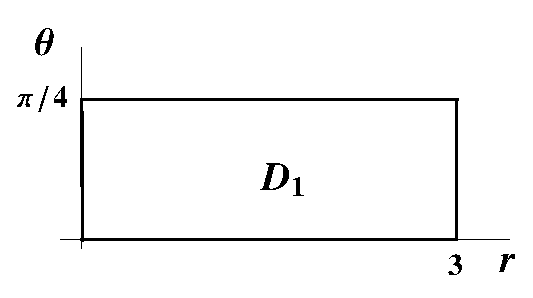
\includegraphics{fig10-1.eps}}\hspace{3cm}
\resizebox{4.5cm}{!}{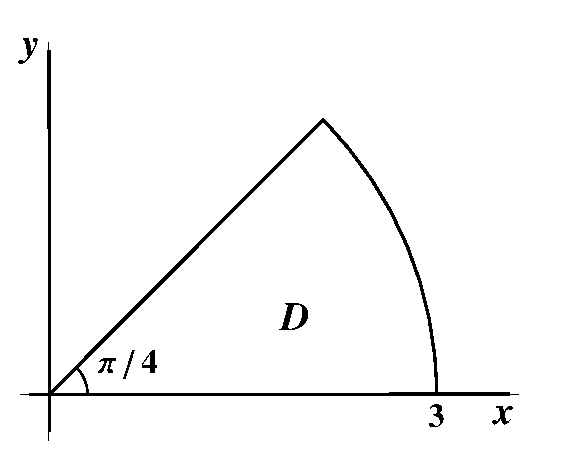
\includegraphics{fig10-2.eps}}
\end{picture}
\end{center}

%*********************************************************************
\vspace*{2cm}

 i les coordenades polars generalitzades rectangles en
seccions el.liptiques.

%*********************************************************************
\vspace*{4cm}
\begin{center}
\begin{picture}(0,0)(170,30)
\resizebox{4.cm}{!}{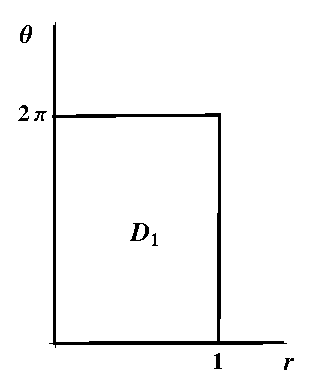
\includegraphics{fig10-3.eps}}\hspace{3cm}
\resizebox{4.5cm}{!}{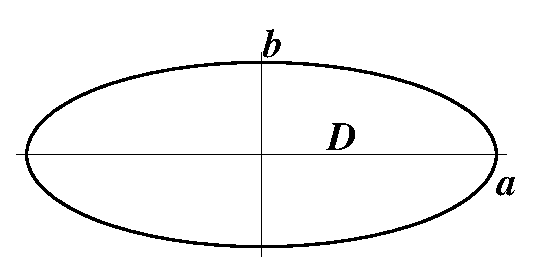
\includegraphics{fig10-4.eps}}
\end{picture}
\end{center}

%*********************************************************************
\vspace*{1cm}

Podem donar ara el \textbf{teorema del canvi de variable} que ens
permetr{\`a} canviar de varia-bles quan sigui convenient.\\

\begin{teorema}
Sigui $\ g:D_1\to D\ $ una transformaci{\'o} regular i sigui $\ f:D\to
\R\ $ una funci{\'o} integrable. Llavors

$$\int_D f=\int_{D_1} (f\circ g)|det(J_g)|$$
\end{teorema}

\begin{observacio}
En el cas particular de les coordenades polars tendrem que:

$$\int_D f(x,y)\,dx\,dy=\int_{D_1} f(r\cos \theta,r\sin \theta)\, r\,dr\,d \theta$$
\end{observacio}

\begin{exemple}
Calculau l'{\`a}rea de la regi{\'o} del primer quadrant $D$ limitada per les
circumfer{\`e}ncies $\ x^2+y^2=a^2\,,\ x^2+y^2=b^2\,,\ $ amb $\,
0<a<b\,.$
\end{exemple}

%*********************************************************************
\vspace*{2.5cm}
\begin{center}
\begin{picture}(0,0)(70,30)
\resizebox{4.5cm}{!}{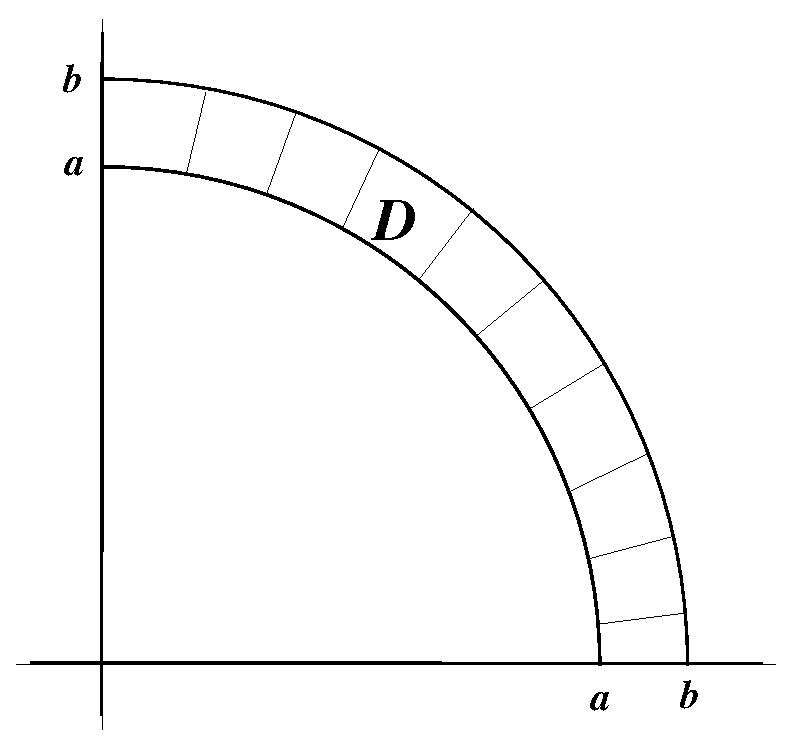
\includegraphics{fig11.eps}}
\end{picture}
\end{center}

%*********************************************************************
\vspace*{1cm}

Sabem que l'{\`a}rea es pot calcular per $\ \displaystyle
A(D)=\int_D\,dx\,dy\,.$

Si consideram les coordenades polars els c{\`a}lculs seran m{\'e}s
senzills:\\

\hspace*{1cm}$\ \displaystyle
A(D)=\int_{D_1}\,r\,dr\,d\theta=\int_0^{\pi/2}\left(
\int_a^b\,r\,dr\right)d\theta=
\int_0^{\pi/2}\left[\frac{r^2}{2}\right]_a^b d\theta=$\\\\

\hspace*{1cm}$\
\displaystyle\frac{1}{2}\int_0^{\pi/2}(b^2-a^2)d\theta
=\frac{1}{2}\left[(b^2-a^2)\theta\right]_0^{\pi/2}=\frac{1}{2}(b^2-a^2)\frac{\pi}{2}
=\frac{\pi}{4}(b^2-a^2)\,.$\\

\begin{exemple}
Calculau  $I=\displaystyle\int_D\, xy\,dx\,dy\ $ on $D$ es {\'e}s
paral.lelogram de la p{\`a}gina 6.
\end{exemple}

Com hem comentat abans aquest domini {\'e}s una uni{\'o} de dues regions o
b{\'e} de tipus 1 o b{\'e} de tipus 2, llavors per fer la integral haur{\'\i}em
de fer la suma de dues integrals.\\

\hspace*{1cm} $I=\displaystyle\int_{D_1}\, xy\,dx\,dy\ +\int_{D_2}\,
xy\,dx\,dy\,,\ \ \ \ \ $ o b{\'e} $\ \ \ \ \ \displaystyle
I=\int_{D_3}\, xy\,dx\,dy+\int_{D_4}\, xy\,dx\,dy\,. $

\newpage
En canvi si consideram les variables $\ s=x+y,\ t=x-y\,,\ $ el
paral.lelogram $D$ es transforma en el quadrat $\ D_1\ $


%*********************************************************************
\vspace*{1.5cm}
\begin{center}
\begin{picture}(0,0)(130,30)
\resizebox{4.cm}{!}{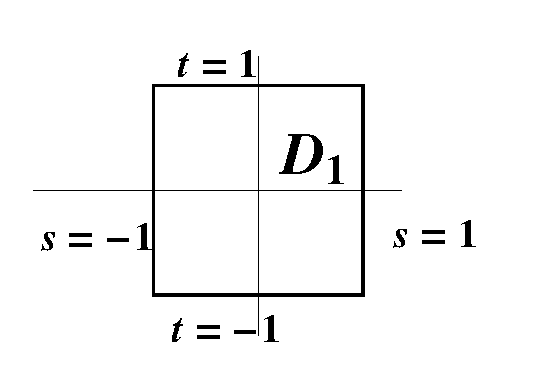
\includegraphics{fig13.eps}}
\end{picture}
\end{center}

%*********************************************************************
\vspace*{1cm}

Llavors considerant el canvi de variables invers $\ x=(s+t)/2,\,
y=(s-t)/2\ $ podem definir la transformaci{\'o} regular $\
g(s,t)=((s+t)/2, (s-t)/2)\,. $ El determinant de la matriu jacobiana
del canvi de variables ve donat per:\\

\hspace*{1cm} $\det(J_g)=
\begin{vmatrix}
1/2 & 1/2\\ 1/2 & -1/2
\end{vmatrix}=|-1/2|=1/2\,.$ Per tant si aplicam el teorema del
canvi\\

 de variable per a calcular la integral tenim:\\

\hspace*{1cm} $I=\displaystyle\int_{D_1}\,
\left(\frac{s+t}{2}\right)\left(\frac{s-t}{2}\right)\frac{1}{2}\,ds\,dt=
\frac{1}{8}\int_{-1}^1\left(\int_{-1}^1(s^2-t^2)ds\right)dt=$\\\\


\hspace*{1cm}
$\displaystyle\frac{1}{8}\int_{-1}^1\left[\frac{s^3}{3}- s
t^2\right]_{-1}^1dt= \frac{2}{8}\int_{-1}^1(\frac{1}{3}-  t^2)dt=
\frac{1}{4}\left[\frac{1}{3}t-\frac{t^3}{3}\right]_{-1}^1=0\,.$

\end{document}
